%%%%%%%%%%%%%%%%%%%%%%%%%%%%%%%%%%%%%%%%%%%%%%%%%%%%%%%%%%%%%%%%%%%%%%%%%%%
%
% Generic template for TFC/TFM/TFG/Tesis
%
% $Id: manual.tex,v 1.8 2014/01/08 22:56:03 macias Exp $
%
% By:
%  + Javier Mac�as-Guarasa. 
%    Departamento de Electr�nica
%    Universidad de Alcal�
%  + Roberto Barra-Chicote. 
%    Departamento de Ingenier�a Electr�nica
%    Universidad Polit�cnica de Madrid   
% 
% Based on original sources by Roberto Barra, Manuel Oca�a, Jes�s Nuevo,
% Pedro Revenga, Fernando Herr�nz and Noelia Hern�ndez. Thanks a lot to
% all of them, and to the many anonymous contributors found (thanks to
% google) that provided help in setting all this up.
%
% See also the additionalContributors.txt file to check the name of
% additional contributors to this work.
%
% If you think you can add pieces of relevant/useful examples,
% improvements, please contact us at (macias@depeca.uah.es)
%
% Copyleft 2013
%
%%%%%%%%%%%%%%%%%%%%%%%%%%%%%%%%%%%%%%%%%%%%%%%%%%%%%%%%%%%%%%%%%%%%%%%%%%%

\chapter{Planos el�ctricos}
\label{cha:planos_electricos}

Los planos electr�cos y documentaci�n de fabricaci�n de la tarjetas electr�nicas desarrolladas se encuentra en el repositorio \texttt{hardware} del equipo Eurobotics Engineering en GitHub. 

Este repositorio es accesible desde la direcci�n web: https://github.com/eurobotics.

El CD-ROM adjunto a este libro contiene una copia de este repositorio.

Adem�s, en este cap�tulo, se ha considerado oportuno incluir una versi�n impresa los planos el�ctricos de las tarjetas electr�nicas.

\begin{figure}[h]
\centering
\includegraphics[width=.8\textwidth]{fotos_tarjetas/eurobotics_boards}
\end{figure}

\pagebreak
\section{Tarjeta \emph{dspic33\_protoboard}}

Dise�o electr�nico y PCB: Javier Bali�as Santos

\vspace*{\fill}
\begin{center}
\includegraphics[width=.9\textwidth]{fotos_tarjetas/dspic33_protoboard}
\end{center}
\vspace*{\fill}

\pagebreak
\includepdf[scale=.95, pages=-, angle=90]{./appendix/dspic33_protoboard.pdf}

\pagebreak
\section{Tarjeta \emph{mainboard\_v02}}

Dise�o electr�nico y PCB: Javier Bali�as Santos

\vspace*{\fill}
\begin{center}
\includegraphics[width=.8\textwidth]{fotos_tarjetas/mainboard_v01_v02}
\end{center}
\vspace*{\fill}

\pagebreak
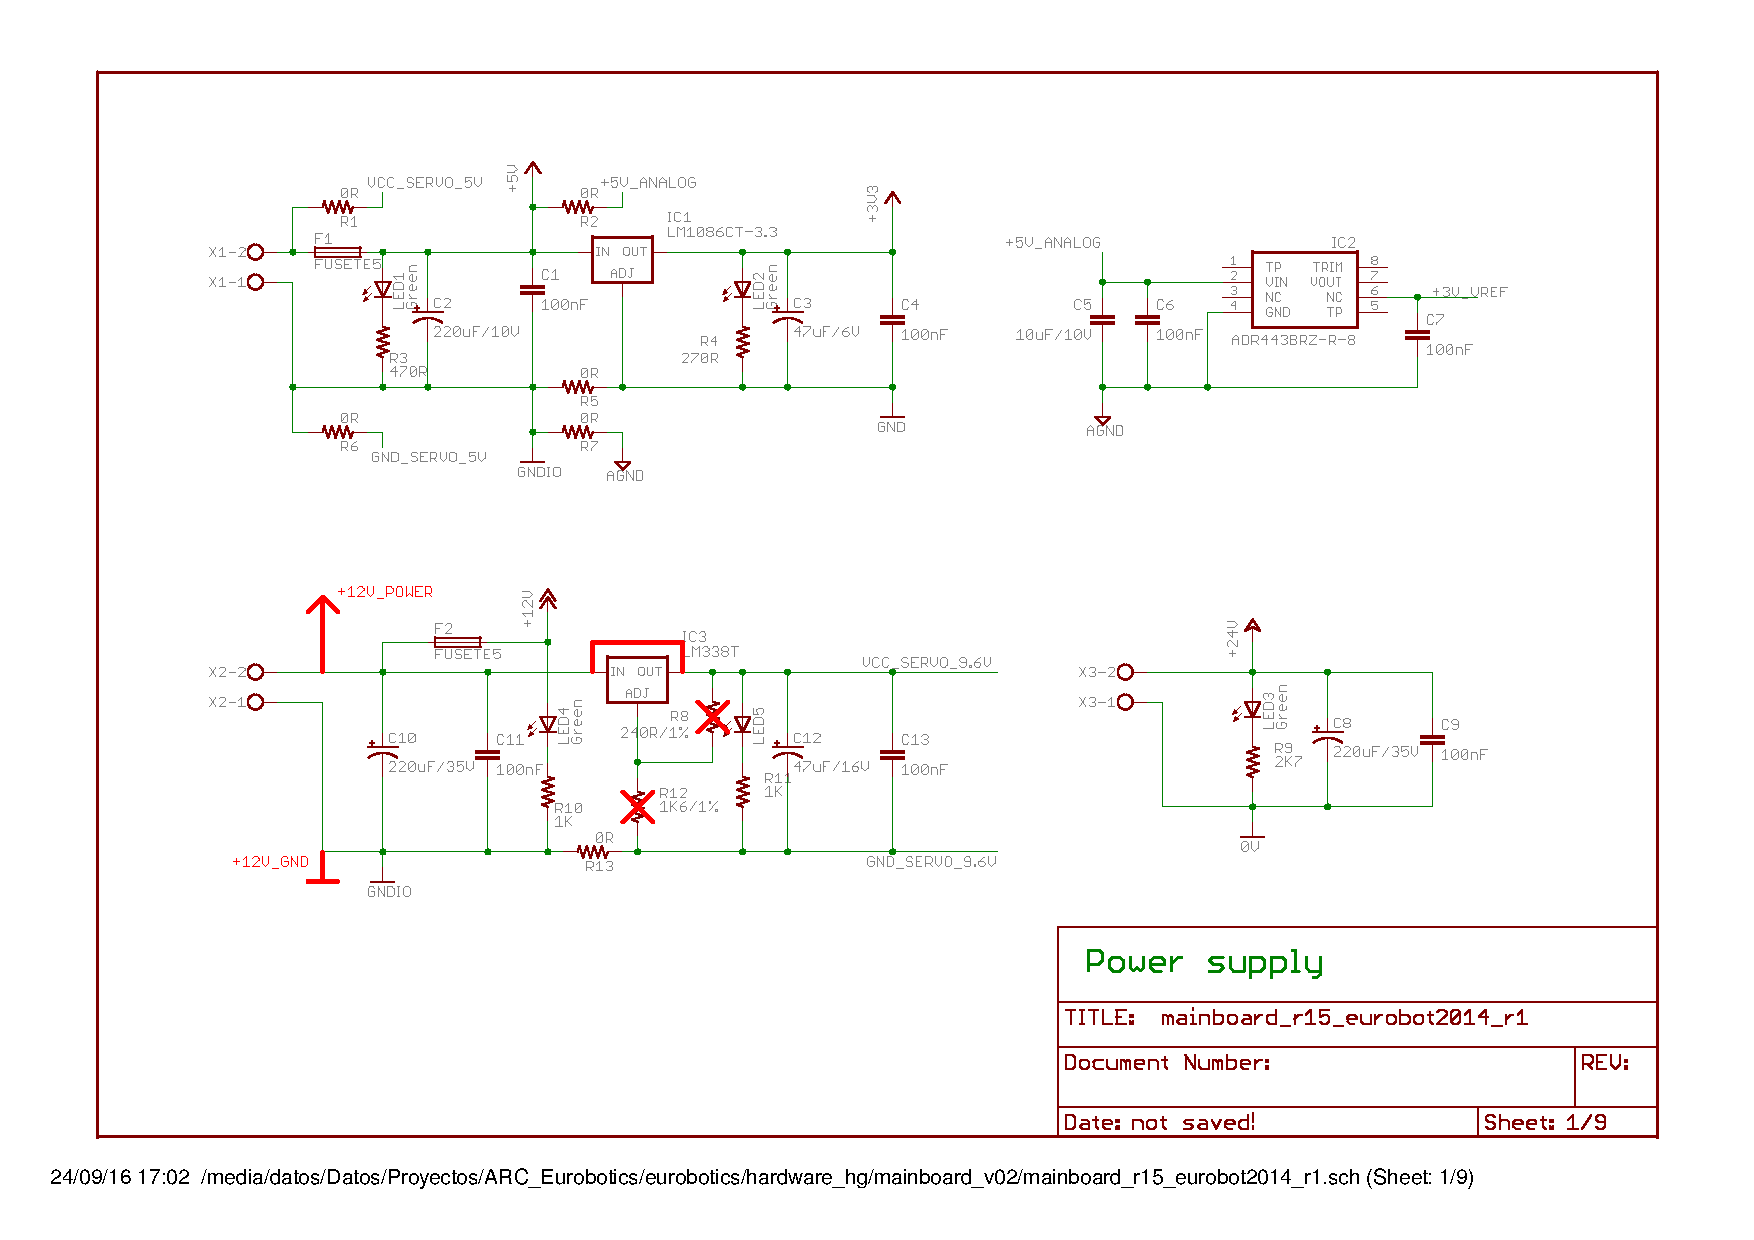
\includepdf[scale=.95, pages=-, angle=90]{./appendix/mainboard_v02.pdf}

\pagebreak
\section{Tarjeta \emph{mainboard\_v03}}

Dise�o electr�nico: Javier Bali�as Santos

Dise�o PCB: Rub�n Espino San Jos�

\vspace*{\fill}
\begin{center}
\includegraphics[width=.8\textwidth]{fotos_tarjetas/mainboard_v03}
\end{center}
\vspace*{\fill}

\pagebreak
\includepdf[scale=.95, pages=-, angle=0]{./appendix/mainboard_v03.pdf}

\pagebreak
\section{Tarjeta \emph{switchboard}}

Dise�o electr�nico y PCB: Javier Bali�as Santos

\vspace*{\fill}
\begin{center}
\includegraphics[width=.8\textwidth]{fotos_tarjetas/switchboard}
\end{center}
\vspace*{\fill}

\pagebreak
\includepdf[scale=.95, pages=-, angle=90]{./appendix/switchboard.pdf}

\pagebreak
\section{Tarjeta \emph{sensorboard}}

Dise�o electr�nico y PCB: Javier Bali�as Santos

\vspace*{\fill}
\begin{center}
\includegraphics[width=.8\textwidth]{fotos_tarjetas/sensorboard}
\end{center}
\vspace*{\fill}

\pagebreak
\includepdf[scale=.95, pages=-, angle=90]{./appendix/sensorboard.pdf}

\pagebreak
\section{Tarjeta \emph{beaconboard}}

Dise�o electr�nico y PCB: Diego Salazar Acucci

\vspace*{\fill}
\begin{center}
\includegraphics[width=.8\textwidth]{fotos_tarjetas/vacuumboard}
\end{center}
\vspace*{\fill}

\pagebreak
\includepdf[scale=.95, pages=-, angle=0]{./appendix/vacuumboard.pdf}

\pagebreak
\section{Tarjeta \emph{vacuumboard}}

Dise�o electr�nico: Javier Bali�as Santos

Dise�o PCB: Rub�n Espino San Jos�

\vspace*{\fill}
\begin{center}
\includegraphics[width=.8\textwidth]{fotos_tarjetas/vacuumboard}
\end{center}
\vspace*{\fill}

\pagebreak
\includepdf[scale=.95, pages=-, angle=0]{./appendix/vacuumboard.pdf}





%%% Local Variables:
%%% TeX-master: "../book"
%%% End:

